\section{Mikrofon}
Til at måle lyden er der valgt en electret condensator mikrofon fra Adafruit, med tilhørende for-forstærker. % https://www.adafruit.com/product/1063
Mikrofonen er designet til at arbejde sammen med Arduino, og har et DC-offset på halvdelen af forsyningspændingen, hvilket gør det nemt at skifte reference. 
Desuden er mikrofonen egnet til optagelse i området $20 Hz - 20 kHz$, hvilket passer fint til projektet. 

\subsection{Sampling af lydinput}
Samplingen af lydsignalet sker gennem Arduinoens ADC. 



\subsection{Antialiasering}
For at undgå aliasering og indstråling af højfrekvent støj, skal mikrofonens output filtreres gennem et anti-aliaseringsfilter.
Filteret er et anden ordens RLC-lavpasfilter, og er realiseret med en knækfrekvens på Nyquist-frekvensen. 
Filteret kunne med fordel laves skarpere end anden orden, men i første omgang er proof of concept mere væsenligt end ydeevne. 
Verifikation og test af filteret kan ses på % ref til test!.

\begin{figure}[H]
	\center
	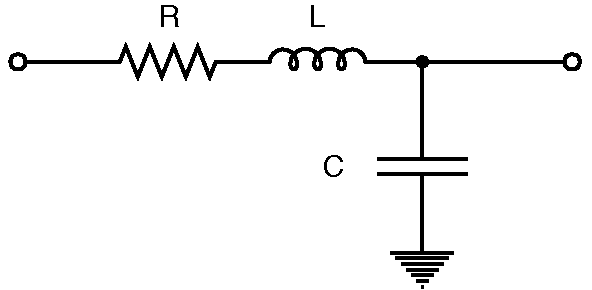
\includegraphics[width=0.3\textwidth]{Figur/RCL_diagram.pdf}
	\caption{RCL-lavpasfilter}
	\label{fig:RCL}
\end{figure}

\section{Frekvensanalyse}



\subsection{Kvalitet af analyse}